\documentclass{article}
\usepackage{graphicx, soul, parskip, amsmath, amssymb}
\usepackage[dvipsnames]{xcolor}
\usepackage[a4paper, margin=0.8in]{geometry}
\usepackage[spanish]{babel}

\setul{0.5ex}{0.3ex}

\newcommand{\ulcolor}[2][Red]{\setulcolor{#1}\ul{#2}}
\newcommand*\sepline{%
  \begin{center}
    \rule[1ex]{.5\textwidth}{.5pt}
  \end{center}}

\title{Ejercicios Adicionales $-$ Fáciles (Resuelto)}
\author{Juani Elosegui}
\date{Diciembre 2024}

\begin{document}
    
    \maketitle

    \section*{\underline{Ejercicio 1}}
        \begin{center}
            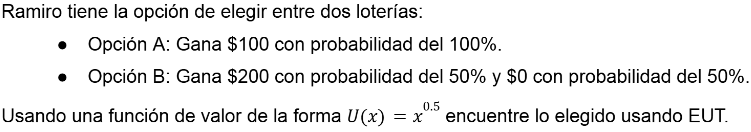
\includegraphics[width=0.8 \linewidth]{figs/adicionales-faciles-uno.png}
        \end{center}
        \textbf{Para resolver esto, tengo que calcular la utilidad esperada, dado que sabemos con qué probabilidad se van a dar los distintos sucesos:}
        \\
        \\
        \(EUT_{A} = P($ganar $ \mathdollar 100) \cdot U(\mathdollar 100)\)
        \\
        \(EUT_{A} = 1 \cdot \sqrt{100}\)
        \\
        \(EUT_{A} = 10\)
        \\
        \\
        \(EUT_{B} = P($ganar $ \mathdollar 200) \cdot U(\mathdollar 200) + P($ganar $ \mathdollar 0) \cdot U(\mathdollar 0)\)
        \\
        \(EUT_{B} = 0,5 \cdot \sqrt{200} + 0,5 \cdot \sqrt{0}\)
        \\
        \(EUT_{B} = 0,5 \cdot \sqrt{200}\)
        \\
        \(EUT_{B} \approx 7,07\)
        \\
        \\
        \textbf{Conclusión:}
        \\
        \\
        Como $EUT_{A} > EUT_{B}$, a Ramiro le conviene elegir la opción A.
    
    \section*{\underline{Ejercicio 2}}
        \begin{center}
            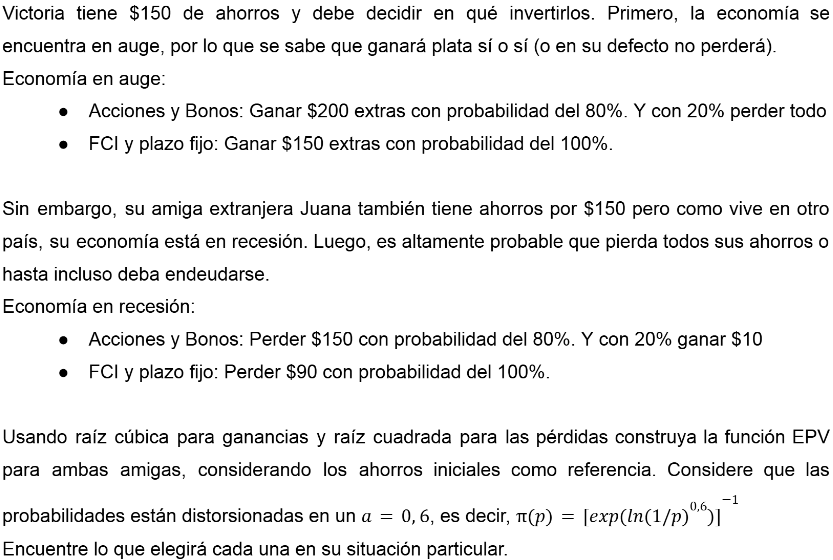
\includegraphics[width=0.8  \linewidth]{figs/adicionales-faciles-dos.png}
        \end{center}
        \textbf{Calculo el EPV para Victoria:}
        \\
        \\
        \(EPV_{V, A/B} = \pi(0,8) \cdot U(\mathdollar 150 + \mathdollar 200) + \pi(0,2) \cdot U(\mathdollar 150 - \mathdollar 150)\)
        \\
        \(EPV_{V, A/B} = \pi(0,8) \cdot \sqrt[3]{\mathdollar 350} + \pi(0,2) \cdot \sqrt[2]{\mathdollar 0}\)
        \\
        \(EPV_{V, A/B} = \pi(0,8) \cdot \sqrt[3]{\mathdollar 350}\)
        \\
        \(EPV_{V, A/B} = \frac{1}{e^{\ln{\frac{1}{0,8}}^{0,6}}} \cdot \sqrt[3]{350}\)
        \\
        \(EPV_{V, A/B} \approx 4,69\)
        \\
        \\
        \(EPV_{V, FCI/PF} = \pi(1) \cdot U(\mathdollar 150 + \mathdollar 150)\)
        \\
        \(EPV_{V, FCI/PF} = \pi(1) \cdot \sqrt[3]{\mathdollar 300}\)
        \\
        \(EPV_{V, FCI/PF} = \frac{1}{e^{\ln{\frac{1}{1}}^{0,6}}} \cdot \sqrt[3]{\mathdollar 300}\)
        \\
        \(EPV_{V, FCI/PF} \approx 6,69\)
        \\
        \\
        \textbf{Calculo el EPV para Juana:}
        \\
        \\
        \(EPV_{J, A/B} = \pi(0,8) \cdot U(\mathdollar 150 - \mathdollar 150) + \pi(0,2) \cdot U(\mathdollar 150 + \mathdollar 10)\)
        \\
        \(EPV_{J, A/B} = \pi(0,8) \cdot \sqrt[2]{\mathdollar 0} + \pi(0,2) \cdot \sqrt[3]{\mathdollar 160}\)
        \\
        \(EPV_{J, A/B} = \pi(0,2) \cdot \sqrt[3]{\mathdollar 160}\)
        \\
        \(EPV_{J, A/B} = \frac{1}{e^{\ln{\frac{1}{0,2}}^{0,6}}} \cdot \sqrt[3]{\mathdollar 160}\)
        \\
        \(EPV_{J, A/B} \approx 1,43\)
        \\
        \\
        \(EPV_{J, FCI/PF} = \pi(1) \cdot U(\mathdollar 150 - \mathdollar 90)\) Queda con menos plata que antes. Por lo tanto, es una pérdida.
        \\
        \(EPV_{J, FCI/PF} = U(\mathdollar 60)\)
        \\
        \(EPV_{J, FCI/PF} = -\sqrt[3]{|60|}\)
        \\
        \(EPV_{J, FCI/PF} \approx -7,75\)
        \\
        \\
        \textbf{Conclusión:}
        \\
        \\
        Victoria eligirá invertir en FCI y Plazo Fijo. Juana decidirá invertir en Acciones y Bonos.

    \section*{\underline{Ejercicio 3}}
      \begin{center}
        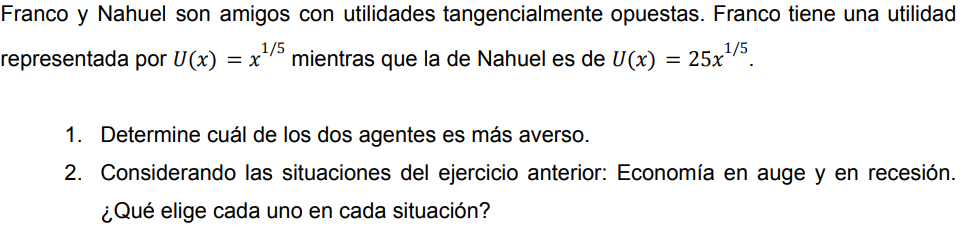
\includegraphics[width=0.8  \linewidth]{figs/adicionales-faciles-tres.png}
      \end{center}
      \textbf{Datos:}
      \\
      \\
      F, \(U_{F}(X) = X^{1/5}\); N, \(U_{N}(X) = 25X^{1/5}\)
      \\
      \\
      \textbf{Para calcular la aversión de cada uno, tengo que usar la fórmula de Arrow-Pratt:}
      \\
      \\
      \(A_{F}(X) = -\frac{U''_{F}}{U'_{F}}\)
      \\
      \(U'_{F} = \frac{1}{5}X^{-4/5}\)
      \\
      \(U''_{F} = \frac{4}{25}X^{-9/5}\)
      \\
      \(\implies A_{F}(X) = -\frac{\frac{4}{25}X^{-9/5}}{\frac{1}{5}X^{-4/5}}\)
      \\
      \(\therefore A_{F}(X) = \frac{4}{5X}\)
      \\
      \\
      \(A_{N}(X) = -\frac{U''_{N}}{U'_{N}}\)
      \\
      \(U'_{N} = 5X^{-4/5}\)
      \\
      \(U''_{N} = -4X^{-9/5}\)
      \\
      \(\implies A_{N}(X) = -\frac{-4X^{-9/5}}{5X^{-4/5}}\)
      \\
      \(\therefore A_{N}(X) = \frac{4}{5X}\)
      \\
      \\
      \textbf{Conclusión:}
      \\
      \\
      Son iguales de aversos.
      \\
      \\
      \textbf{Calculo EUT para cada uno en cada situación para saber qué harían:}
      \\
      \\
      Para Franco:
      \\
      \(EUT_{Franco, A, A/B} = 0,8 \cdot U(150+200) + 0,2 \cdot U(0)\) \\
      \(\implies EUT_{F, A, A/B} = 0,8 \cdot U(150+200)\) \\
      \(\implies EUT_{F, A, A/B} = 0,8 \cdot 350^{1/5}\) \\
      \(\therefore EUT_{F, A, A/B} \approx 2,58\) \\
      \\
      \(EUT_{Franco, A, FCI/PF} = 1 \cdot U(150+150)\) \\
      \(\implies EUT_{F, A, FCI/PF} = 300^{1/5}\) \\
      \(\therefore EUT_{F, A, FCI/PF} \approx 3,12\) \\
      \\
      \(EUT_{Franco, R, A/B} = 0,8 \cdot U(150-150) + 0,2 \cdot U(150+10)\) \\
      \(\implies EUT_{Franco, R, A/B} = 0,2 \cdot 160^{1/5}\) \\
      \(\therefore EUT_{Franco, R, A/B} \approx 2,78\) \\
      \\
      \(EUT_{Franco, R, FCI/PF} = 1 \cdot U(150-90)\) \\
      \(\implies EUT_{Franco, R, FCI/PF} = 60^{1/5}\) \\
      \(\therefore EUT_{Franco, R, FCI/PF} \approx 2,26\) \\
      \\
      Para Nahuel:
      \\
      \(EUT_{Nahuel, A, A/B} = 0,8 \cdot U(150+200) + 0,2 \cdot U(0)\) \\
      \(\implies EUT_{Nahuel, A, A/B} = 0,8 \cdot U(350)\) \\
      \(\implies EUT_{Nahuel, A, A/B} = 0,8 \cdot 25 \cdot 350^{1/5}\) \\
      \(\therefore EUT_{Nahuel, A, A/B} \approx 64,54\) \\
      \\ 
      \(EUT_{Nahuel, A, FCI/PF} = 1 \cdot U(150 + 150)\) \\
      \(\implies EUT_{Nahuel, A, FCI/PF} = U(300)\) \\
      \(\implies EUT_{Nahuel, A, FCI/PF} = 25 \cdot 300^{1/5}\) \\
      \(\therefore EUT_{Nahuel, A, FCI/PF} \approx 78,22\) \\
      \\
      \(EUT_{Nahuel, R, A/B} = 0,8 \cdot U(150 - 150) + 0,2 \cdot U(150 + 10)\) \\
      \(\implies EUT_{Nahuel, R, A/B} = 0,2 \cdot U(160)\) \\
      \(\implies EUT_{Nahuel, R, A/B} = 0,2 \cdot 25 \cdot 160^{1/5}\) \\
      \(\therefore EUT_{Nahuel, R, A/B} \approx 13,8\) \\
      \\
      \(EUT_{Nahuel, R, FCI/PF} = 1 \cdot U(150 - 90)\) \\
      \(\implies EUT_{Nahuel, R, FCI/PF} = U(60)\) \\
      \(\implies EUT_{Nahuel, R, FCI/PF} = 25 \cdot 60^{1/5}\) \\
      \(\therefore EUT_{Nahuel, R, FCI/PF} \approx 56,7\)
      \\
      \\
      \textbf{Conclusión:}
      \\
      \\
      Franco decidirá invertir en FCI y Plazo Fijo en una economía en auge, y en una economía en recesión decidirá invertir en Acciones y Bonos. \\
      Nahuel decidirá invertir en FCI y Plazo Fijo en una economía en auge, y en una economía en recisión también lo hará.

    \section*{\underline{Ejercicio 4}}
      \begin{center}
        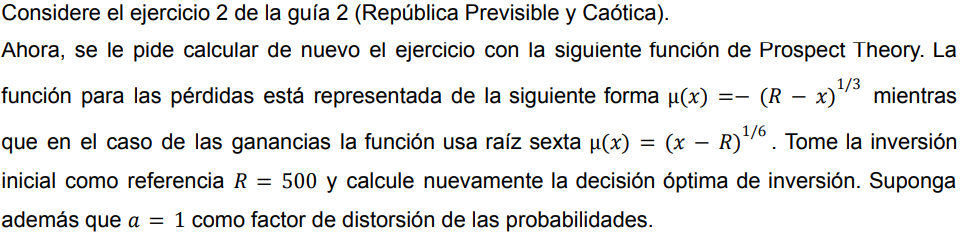
\includegraphics[width=0.8  \linewidth]{figs/adicionales-faciles-cuatro.png}
      \end{center}
      \begin{center}
        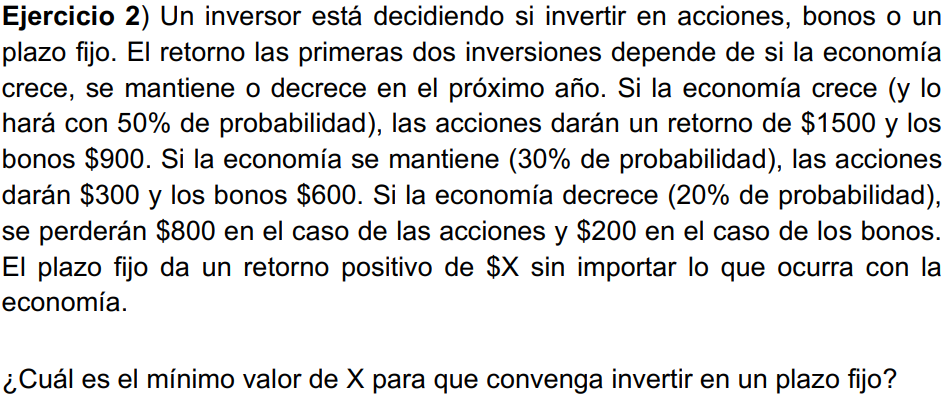
\includegraphics[width=0.8  \linewidth]{figs/adicionales-faciles-cuatro-b.png}
      \end{center}
      \textbf{Momento de las cuentas \ulcolor[Red]{(no sé lo que estoy haciendo)}:}
      \\
      \\
      Sea \(R = 500\) y la función de Prospect Theory definida como:
      \[
        \mu(x) =
        \begin{cases} 
          -(500-x)^{1/3} & \text{si } x \leq 500, \\ 
          (x-500)^{1/6} & \text{si } x > 500.
        \end{cases}
      \]
      \(PV_{Acciones} = 0,5 \cdot \mu(1500) + 0,3 \cdot \mu(300) + 0,2 \cdot \mu(-800)\) \\
      \(PV_{Acciones} = 0,5 \cdot (1500-500)^{1/6} + 0,3 \cdot -(500 - 300)^{1/3} + 0,2 \cdot -(500 - (-800))^{1/3}\) \\
      \(PV_{Acciones} = 0,5 \cdot (1000)^{1/6} + 0,3 \cdot -200^{1/3} + 0,2 \cdot -(1300)^{1/3}\) \\
      \(PV_{Acciones} = 0,5 \cdot 1000^{1/6} - 0,3 \cdot 200^{1/3} - 0,2 \cdot 1300^{1/3}\) \\
      \(PV_{Acciones} \approx -2,36\) \\
      \\
      \(PV_{Bonos} = 0,5 \cdot \mu(900) + 0,3 \cdot \mu(600) + 0,2 \cdot \mu(-200)\) \\
      \(PV_{Bonos} = 0,5 \cdot (900-500)^{1/6} + 0,3 \cdot (600-500)^{1/6} + 0,2 \cdot -(500-(-200))^{1/3}\) \\
      \(PV_{Bonos} = 0,5 \cdot 400^{1/6} + 0,3 \cdot 100^{1/6} - 0,2 \cdot 700^{1/3}\) \\
      \(PV_{Bonos} \approx 0,23\) \\
      \\
      \textbf{Conclusión:}
      \\
      \\
      Conviene invertir en bonos.  
\end{document}